\documentclass[11pt,a4paper]{article}

% ---------------------------------------------------------------------------
% Packages
% ---------------------------------------------------------------------------
\usepackage[utf8]{inputenc}
\usepackage[T1]{fontenc}
\IfFileExists{lmodern.sty}{\usepackage{lmodern}}{}  % always present on Overleaf
\usepackage[margin=2.5cm]{geometry}
\usepackage{amsmath}
\usepackage{graphicx}
\usepackage{booktabs}
\usepackage{makecell}
\usepackage[font=small,labelfont=bf]{caption}
\usepackage[round,authoryear]{natbib}
\usepackage{xcolor}
\usepackage{enumitem}
\usepackage[section]{placeins}  % keep figures and tables inside their own section
\usepackage[colorlinks=true,linkcolor=blue!50!black,citecolor=blue!50!black,urlcolor=blue!50!black]{hyperref}

\graphicspath{{figures/}}

% Visible placeholder for text still to be written; remove before submission.
\newcommand{\todo}[1]{\textcolor{red!70!black}{\textbf{[TODO:} #1\textbf{]}}}

% ---------------------------------------------------------------------------
% Front matter
% ---------------------------------------------------------------------------
\title{Confident but Wrong: Calibration and Selective Automation of Bearing Fault Diagnosis Under Artificial-to-Real Damage Shift}
\author{%
  Yam Malla\thanks{Corresponding author. Email: \href{mailto:yammalla09@gmail.com}{yammalla09@gmail.com}}
  \and
  Bhuwan Karki\thanks{Email: \href{mailto:bhuwan.karki7@gmail.com}{bhuwan.karki7@gmail.com}}%
}
\date{}

\begin{document}

\maketitle

\begin{abstract}
Automated bearing fault diagnosis relies on trustworthy predictive confidence to determine when the system should
defer to a human operator. Machine-learning classifiers are usually trained and calibrated on artificial defects but
must ultimately diagnose naturally developing damage, such as fatigue pitting. Whether their confidence can still be
trusted after this shift has received little attention. This study evaluates whether confidence thresholds, post-hoc
calibration and conformal prediction guarantees transfer from artificial to real damage. Random Forest, support vector
machine and XGBoost classifiers on envelope-spectrum features and a one-dimensional convolutional neural network
(1D-CNN) on raw vibration are trained and calibrated on artificially damaged Paderborn bearings and tested on real
damage, with bearing-level splits, 105 choices of calibration bearings and four operating conditions. At the main
operating condition, the feature-based models are close to calibrated on unseen artificial bearings (expected
calibration error 0.01--0.09), but on real damage accuracy drops from 0.88--0.91 to about 0.69, and thresholds tuned
for a 5\,\% target error give 24--27\,\% error, exceeding the target for every calibration choice. Neither temperature
scaling nor isotonic regression corrects this overconfidence, and conformal coverage falls to 0.65--0.68 against a
nominal 0.90. The failures stem largely from ``silent'' real-damage bearings lacking distinct fault-frequency peaks in
their envelope spectra, which the models confidently call healthy; they recur at the other operating conditions, more
mildly where the features are weaker. Calibrating on two labelled real bearings per class reduces the error to
0.10--0.11 but meets the target in only about half of the trials and automates far fewer cases. The 1D-CNN fails even
on unseen artificial bearings (0.46 accuracy vs.\ 0.98 under random window splits), and adaptive batch normalisation
(AdaBN) on unlabelled real-damage data raises its real-damage accuracy from 0.43 to 0.51 but not the reliability of
its confidence. Consequently, safety-critical automation thresholds must be evaluated on real-damage data with strict
bearing-level validation, and results reported per bearing.
\end{abstract}


\section{Introduction}
\label{sec:introduction}

\todo{About 800 words. Planned content (see \texttt{docs/paper/outline.md}):}
\begin{itemize}[nosep]
  \item Why bearing fault diagnosis is automated, and why automation needs trustworthy confidence: a system should act
        alone only when it is likely right and otherwise ask a human.
  \item Models are usually developed on artificially made faults but deployed on naturally developed damage.
  \item Research questions: how much accuracy and calibration degrade from artificial to real damage; whether
        post-hoc calibration and conformal prediction fitted on artificial data still hold; how many labelled real
        bearings restore trustworthy confidence.
  \item Contributions (from the outline): artificial$\to$real evaluation of calibration and selective automation;
        thresholds fail in every rotation; conformal under-coverage; silent bearings; real-bearing calibration;
        feature ablation.
\end{itemize}

\section{Related work}
\label{sec:related}

\todo{About 700 words, after verifying every reference. Planned subsections:}
\begin{itemize}[nosep]
  \item Bearing benchmarks and evaluation pitfalls \citep{smith2015,lessmeier2016}; recording-level evaluation
        \citep{gonzalezgarcia2026}.
  \item Domain shift in fault diagnosis, including the artificial-to-real gap reported by \citet{lessmeier2016}.
  \item Calibration and conformal prediction \citep{guo2017,ovadia2019,angelopoulos2023,tibshirani2019}, and their
        first use for vibration-based bearing classification \citep{gonzalezgarcia2026}.
  \item Selective classification \citep{geifman2017}.
\end{itemize}

\section{Methods}
\label{sec:methods}

\subsection{Dataset}

We use the Paderborn University KAt bearing dataset \citep{lessmeier2016,katdatacenter}, which contains measurements
of deep-groove ball bearings (type 6203) in an electromechanical drive test rig. Its distinguishing feature for this study is that
it contains both \emph{artificially damaged} bearings (damage introduced by electric discharge machining, drilling or
electric engraving) and bearings with \emph{real damage} that developed during accelerated lifetime tests. We use the
vibration signal (sampled at 64\,kHz). The main analysis uses the operating condition \texttt{N15\_M07\_F10}:
1{,}500\,rpm shaft speed, 0.7\,Nm load torque and 1{,}000\,N radial force. To test whether the findings depend on
this choice, we repeat the evaluation at the dataset's three other conditions: lower load torque (0.1\,Nm), lower
radial force (400\,N) and lower speed (900\,rpm), with the other two parameters unchanged
(Section~\ref{sec:conditions}). Each bearing has 20 recordings of 4\,s per condition.

We consider three classes---healthy, inner-race fault and outer-race fault---and use 29 bearings: 6 healthy, 12 with
artificial damage (7 outer race, 5 inner race) and 11 with real damage (5 outer race, 6 inner race): healthy
K001--K006; artificial outer race KA01, KA03, KA05--KA09; artificial inner race KI01, KI03, KI05, KI07, KI08; real
outer race KA04, KA15, KA16, KA22, KA30; real inner race KI04, KI14, KI16--KI18, KI21. The real damage is fatigue
pitting in nine bearings and plastic deformation (indentations) in KA15 and KA30, with a documented extent of level 1
except for KA16 and KI18 (level 2) and KI16 (level 3) \citep{lessmeier2016}. Bearings with combined inner-
and outer-race damage are excluded. Each recording is cut into non-overlapping 1\,s windows (64{,}000 samples). A
few recordings are slightly shorter than 4\,s and give three windows, so each bearing contributes 76--80 windows
(2{,}309 at the main condition, 2{,}305--2{,}308 at the others).

\subsection{Features}
\label{sec:features}

\paragraph{Fault-frequency features (main setting).} For each window we compute the envelope spectrum
\citep{randall2011}: a fourth-order Butterworth band-pass filter (2--10\,kHz) applied forwards and backwards, the
magnitude of the analytic signal (Hilbert transform) with its mean removed, and the magnitude of its discrete
Fourier transform. For the 6203 bearing ($n = 8$ balls, ball diameter $d = 6.75$\,mm, pitch diameter
$D = 28.55$\,mm, contact angle $0^\circ$) at shaft frequency $f_r = 25$\,Hz, the ball-pass frequencies of the outer
race (BPFO) and of the inner race (BPFI) are
\begin{equation}
  \begin{aligned}
    \mathrm{BPFO} &= \frac{n}{2}\left(1 - \frac{d}{D}\right) f_r \approx 76.4\,\mathrm{Hz},\\
    \mathrm{BPFI} &= \frac{n}{2}\left(1 + \frac{d}{D}\right) f_r \approx 123.6\,\mathrm{Hz}.
  \end{aligned}
\end{equation}
At 900\,rpm ($f_r = 15$\,Hz) these become 45.8\,Hz and 74.2\,Hz.
For each of BPFO and BPFI and their second harmonics, the feature is the largest envelope-spectrum amplitude within
$\pm 2\,\%$ of the target frequency, which allows for the slip of the rolling elements \citep{randall2011}, divided
by the median envelope-spectrum amplitude between 10 and 500\,Hz (the noise floor). These
four ratios are self-normalised: they compare a peak with the spectrum's own noise floor rather than measuring
absolute vibration level. All four are log-transformed before modelling.

\paragraph{All features (ablation).} The ablation adds five time-domain statistics of the raw window: root mean
square, kurtosis, skewness, crest factor and peak-to-peak amplitude (log-transformed except skewness).

\paragraph{Adaptive band (robustness check).} Because a fixed demodulation band might miss impacts that excite
other resonances, we also select the band per window with the fast kurtogram \citep{antoni2007}, which uses spectral
kurtosis \citep{antoni2006} to find the frequency band, in both centre and width, where a signal is most impulsive.
The kurtosis of the complex envelope is computed for every band of the kurtogram's 1/3-binary grid, with each band's
envelope obtained by band-pass filtering in the frequency domain. Bands are limited to 1--30\,kHz and to widths of
at least 1\,kHz, so that the envelope keeps the second harmonic of the inner-race frequency. The band with the
largest kurtosis is used for demodulation, and the same four fault-frequency features are computed in it.

\paragraph{Order of decisions.} Our first analysis used all nine features. We adopted the fault-frequency features as
the main setting after that analysis showed that the amplitude features generalise poorly to unseen bearings of the
\emph{source} domain (Section~\ref{sec:ablation}). Because this choice was made after seeing results, we report both
settings in full.

\subsection{Bearing-level splits}
\label{sec:splits}

Every bearing belongs to exactly one split, so windows from one bearing never appear in both training and
evaluation. The \emph{source domain} contains the 12 artificially damaged bearings and healthy bearings K001, K002
and K004; the \emph{target domain} contains the 11 real-damage bearings and healthy bearings K003, K005 and K006.

The healthy bearings were assigned with care. Their median kurtosis differs strongly: 13.6--15.8 for K001, K002,
K003 and K006, but 4.2--5.1 for K004 and K005. The high values of the first four suggest an impulsive component
unrelated to bearing damage. We place one low-kurtosis healthy bearing on each side, so that the healthy class itself does not shift between domains.
This assignment was made after inspecting the feature distributions but before any model was trained, and the same
split is used for every operating condition.

From the source domain, one bearing per class is held out as the \emph{calibration set}; the remaining source
bearings form the \emph{training set}. Because results depend strongly on which bearings are held out, we repeat the
whole experiment for every possible choice: $3 \times 5 \times 7 = 105$ rotations (healthy $\times$ inner race
$\times$ outer race). Training sets contain 954--957 windows and calibration sets 237--240. The \emph{test set}---all
14 target-domain bearings, 1{,}115 windows---is the same in every rotation.

\subsection{Classifiers}

We compare three classifiers widely used in condition monitoring, implemented with scikit-learn
\citep{pedregosa2011} and the XGBoost library \citep{chen2016}:
\begin{itemize}[nosep]
  \item \textbf{Random Forest} \citep{breiman2001}: 500 trees, minimum 2 samples per leaf, class-balanced weights.
  \item \textbf{Support vector machine (SVM)} \citep{cortes1995}: radial basis function (RBF) kernel, $C = 1$, $\gamma$ = \texttt{scale},
        standardised inputs, class-balanced weights; probabilities from scikit-learn's internal cross-validated
        Platt scaling \citep{platt1999}.
  \item \textbf{XGBoost}: 300 trees, maximum depth 4, learning rate 0.1, row and column subsampling 0.8,
        class-balanced sample weights.
\end{itemize}
All models use a fixed random seed (0) and are fitted on the training set only. Their hyperparameters were set once to
common values and not tuned, for the same reason as for the network (Section~\ref{sec:cnn}).

\subsection{1D-CNN baseline}
\label{sec:cnn}

To test whether an end-to-end deep network avoids the problems of hand-crafted features, we add a one-dimensional
convolutional neural network (1D-CNN) trained on the raw vibration signal, following the design of WDCNN, a deep
convolutional network with a wide first-layer kernel \citep{zhang2017}. Its input is a 4{,}096-sample segment (64\,ms), standardised to zero mean and unit variance,
which removes the absolute vibration level. A first convolution with 16 filters of length 64 and stride 16 is
followed by four convolutions with kernel length 3 (32, 64, 64 and 64 filters); each of the five convolutions is
followed by batch normalisation, rectified linear unit (ReLU) activation and max-pooling by a factor of 2. A fully
connected layer of 100 units, also with batch normalisation and ReLU, and a three-unit output layer complete the
network. The network is trained for
20 epochs on random segments of the training windows (eight per window and epoch), with Adam (learning rate
$10^{-3}$, weight decay $10^{-4}$, batch size 256) and class-balanced cross-entropy. A window's class probabilities
are the mean softmax output over its 15 non-overlapping segments. These settings were fixed in advance, because no
bearings were left for tuning them without using the calibration or test bearings. One network is trained per
rotation, on that rotation's training bearings, and one per held-out bearing for the in-domain reference; their
probabilities then pass through exactly the same calibration, conformal and selective-automation procedures as those
of the other classifiers. As a sanity check, the network and the feature-based classifiers are also trained once on a
random 80/20 split of the source bearings' windows, in which every bearing appears in both the training and the test
set.

\paragraph{Domain adaptation (AdaBN).} To test whether unsupervised domain adaptation makes the network's confidence
trustworthy, we apply adaptive batch normalisation \citep[AdaBN;][]{li2018}, which the WDCNN authors used to adapt
to changing loads \citep{zhang2017}. AdaBN keeps all learned weights and replaces the means and variances stored in
all batch-normalisation layers with those of unlabelled target-domain data, so that every layer's inputs are
standardised in the new domain as they were in the source domain. The adaptation is held out by bearing: each target
bearing is predicted by the rotation's network with statistics estimated on the windows of the other 13 target
bearings, so no test bearing contributes to its own adaptation, and no labels are used. Calibration bearings belong to
the source domain and keep the original statistics, so thresholds and calibrators are fitted exactly as without
adaptation.

\subsection{Calibration and conformal prediction}

Post-hoc calibrators are fitted on the calibration set's predicted probabilities:
\begin{itemize}[nosep]
  \item \textbf{Temperature scaling} \citep{guo2017}: probabilities are rescaled as
        $\mathrm{softmax}(\log \hat{p} / T)$, with a single $T$ chosen to minimise the negative log-likelihood.
  \item \textbf{Isotonic regression} \citep{zadrozny2002}: one-vs-rest isotonic regression per class, followed by
        renormalisation.
\end{itemize}
The uncalibrated (``raw'') probabilities are reported as a third option.

\emph{Split conformal prediction} \citep{vovk2005,angelopoulos2023} uses the non-conformity score
$1 - \hat{p}(y)$ of the true class $y$, computed from the uncalibrated probabilities of the calibration set. The
threshold is the $(k+1)$-th smallest of the $n$ calibration scores, with $k = \lceil (n+1)(1-\alpha) \rceil$ and
$\alpha = 0.1$ (nominal coverage 0.90); this is one rank above the standard split-conformal quantile and therefore
slightly conservative. A class enters a test window's prediction set when its score is at or below the threshold, so sets may
be empty. We use a single threshold (\emph{marginal}) and one threshold per class (\emph{class-conditional},
Mondrian).

\subsection{Selective automation}
\label{sec:selective}

A deployed system acts automatically only when its confidence (the largest class probability) reaches a threshold,
and passes the remaining cases to a human \citep{geifman2017}. For an error target $\varepsilon$ (1\,\% or 5\,\%),
we choose, on the calibration set's (calibrated) probabilities, the lowest threshold whose automatically decided
calibration windows have an error rate of at most $\varepsilon$; ties in confidence are kept together. We then apply this threshold to the test set and report the
\emph{automation rate} (share of test windows decided automatically) and the \emph{automated error} (error rate among
them). As a reference, the \emph{best possible automation} is the automation rate obtained when the threshold is
chosen on the test set itself. If no threshold meets the target on the calibration set, nothing is automated; when we
report how often the target is exceeded across rotations, we count only rotations in which at least one test window
is automated.

\subsection{Metrics}

We report accuracy and per-class recall; the expected calibration error (ECE; top-label, 10 equal-width confidence
bins); the area under the risk--coverage curve (AURC), i.e.\ the mean error among the $k$ most confident windows over
all $k$ \citep{geifman2019}; and conformal empirical coverage and mean prediction-set size. Errors on real damage are
divided into missed faults (a damaged bearing predicted healthy), false alarms (a healthy bearing predicted damaged)
and confusions between the two fault types.

\subsection{In-domain reference}

To separate the artificial-to-real shift from the difficulty of generalising to any unseen bearing, we also evaluate
each classifier on the source domain by leave-one-bearing-out. Each of the 15 source bearings is predicted by a model
trained on the other 14, and metrics are computed on the pooled predictions (raw probabilities).

\subsection{Uncertainty of the estimates}
\label{sec:bootstrap}

With only 3--6 test bearings per class, bearing-to-bearing variation dominates the uncertainty. We therefore use a
hierarchical bootstrap with 2{,}000 draws. Each draw picks one of the 105 rotations at random, then resamples the test
bearings with replacement within each class, keeping the number of bearings per class (3 healthy, 6 inner race,
5 outer race). All metrics are recomputed on the windows of the resampled bearings, with that rotation's calibrators
and thresholds, and we report the mean and the
2.5th--97.5th percentile interval.

\subsection{Calibrating on labelled real bearings}
\label{sec:realcal}

To test whether a small amount of labelled target data restores trustworthy confidence, we move $n = 1$ or 2
target-domain bearings per class from the test set into a separate calibration set, using 50 random selections per
$n$, each combined with a randomly chosen rotation. The classifier is always trained on that rotation's source
training set. We compare three calibration sets, all evaluated on the \emph{same remaining test bearings}:
\emph{source} (the rotation's held-out source bearings), \emph{target} (only the $n$ target bearings per class) and
\emph{combined} (both). Calibrators, conformal thresholds and automation thresholds are fitted on each calibration set
in turn. This experiment is run for the main operating condition only.

\subsection{Implementation}

The pipeline is implemented in Python using NumPy 2.2.6, SciPy 1.15.3, pandas 2.3.3, scikit-learn 1.7.2 and XGBoost
3.2.0; the 1D-CNN is implemented in PyTorch 2.11.0 and was trained on a GPU in Google Colab. Code,
configuration and all result tables are available at \url{https://github.com/amritmalla/bearing-uq-artificial-to-real}; every figure and table can be regenerated
from the Paderborn recordings with the scripts listed in the repository README.

\section{Results}
\label{sec:results}

Unless stated otherwise, results are for the main operating condition and the fault-frequency features, calibrated
results use temperature scaling, and
values are bootstrap means with 95\,\% intervals in brackets (Section~\ref{sec:bootstrap}); values given as medians or
means over rotations are labelled as such.

% Generated by scripts/build_paper_assets.py -- do not edit by hand.
\begin{table*}[t]
\centering
\small
\begin{tabular}{lccc}
\toprule
Metric & \textbf{Random Forest} & \textbf{SVM} & \textbf{XGBoost} \\
\midrule
In-domain accuracy & 0.91 & 0.88 & 0.91 \\
In-domain ECE & 0.01 & 0.09 & 0.06 \\
Real accuracy & 0.69 [0.52, 0.86] & 0.69 [0.50, 0.86] & 0.70 [0.52, 0.85] \\
Real ECE & 0.19 [0.05, 0.35] & 0.17 [0.04, 0.35] & 0.20 [0.06, 0.35] \\
AURC & 0.15 [0.04, 0.34] & 0.15 [0.03, 0.34] & 0.15 [0.04, 0.33] \\
Error at 5\% target & 0.27 [0.10, 0.46] & 0.24 [0.07, 0.45] & 0.26 [0.09, 0.44] \\
Automated at 5\% target & 0.87 [0.66, 1.00] & 0.82 [0.47, 1.00] & 0.86 [0.69, 1.00] \\
Best possible automation at 5\% target & 0.32 [0.00, 0.71] & 0.31 [0.03, 0.75] & 0.30 [0.00, 0.72] \\
Conformal coverage (nominal 0.90) & 0.65 [0.43, 0.84] & 0.68 [0.45, 0.87] & 0.67 [0.45, 0.85] \\
\bottomrule
\end{tabular}
\caption{Main results (fault-frequency features, temperature scaling). In-domain: leave one source bearing out, raw probabilities. Real damage: mean [95\,\% interval] from 2,000 bootstrap draws over calibration rotations and test bearings.}
\label{tab:main}
\end{table*}


\subsection{The artificial-to-real gap}

On unseen artificial bearings, all three classifiers generalise well: leave-one-bearing-out accuracy is 0.91
(Random Forest), 0.88 (SVM) and 0.91 (XGBoost), and their probabilities are close to calibrated (ECE 0.01, 0.09 and
0.06; Table~\ref{tab:main}). On real damage, accuracy falls to 0.69--0.70 for every model (e.g.\ Random Forest
0.69 [0.52, 0.86]), and ECE rises to 0.17--0.20 after temperature scaling. The wide intervals reflect how strongly
individual real bearings differ (Section~\ref{sec:silent}).

Recall on real damage differs by class: 0.82--0.85 for healthy bearings, 0.73 for inner-race and 0.56--0.57 for
outer-race damage (means over rotations). Outer-race damage, the easiest class on artificial bearings (0.97--0.99
in-domain), is the hardest on real ones.

\subsection{Confidence thresholds chosen on artificial damage do not transfer}

Fig.~\ref{fig:riskcoverage} shows the error among automatically decided cases as more cases are automated. On
unseen artificial bearings, the best possible threshold keeps the error at or below 5\,\% while automating 81--91\,\% of cases.
On real damage, the best possible threshold keeps the error at or below 5\,\% for only 25--30\,\% of cases (median over
rotations, uncalibrated probabilities; the bootstrap means after temperature scaling in Table~\ref{tab:main} are
0.30--0.32).

\begin{figure*}[t]
  \centering
  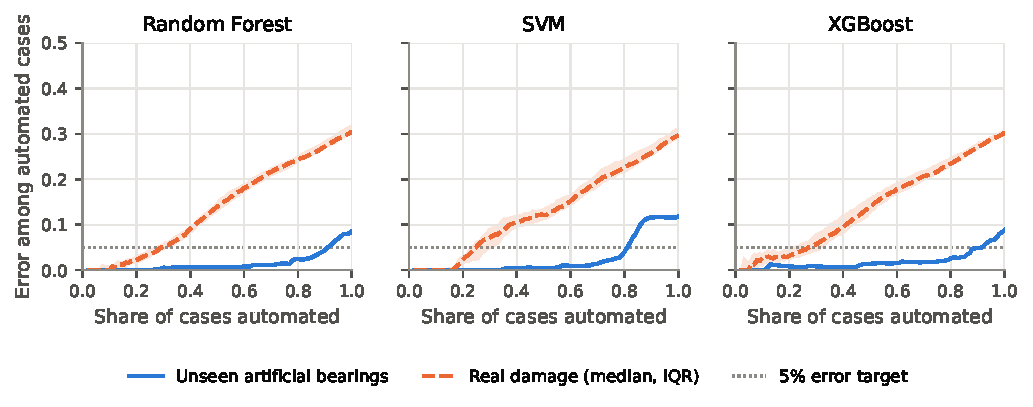
\includegraphics[width=\textwidth]{fig1_risk_coverage}
  \caption{Error among automatically decided cases as a function of the share of cases automated (most confident
    first), for unseen artificial bearings (leave one bearing out; solid) and real damage (dashed; median and
    interquartile range over 105 rotations; uncalibrated probabilities). Dotted line: 5\,\% error target. With the best possible threshold, the
    models automate 81--91\,\% of unseen artificial-bearing cases at or below 5\,\% error, but only 25--30\,\% of
    real-damage cases.}
  \label{fig:riskcoverage}
\end{figure*}

In deployment the threshold must be chosen without real-damage labels. A threshold chosen on the calibration set for
a 5\,\% error target automates 82--87\,\% of real-damage cases, with an error of 0.24--0.27 among them
(Table~\ref{tab:main}). The lower ends of the 95\,\% intervals (0.07--0.10) are still above the target, and the
target is exceeded in all 105 rotations for every model. A stricter 1\,\% target does not solve the problem: about
half of the cases are still automated (0.48--0.53), with an error of 0.13--0.15 (means over rotations).

The reliability diagrams in Fig.~\ref{fig:reliability} show why: on real damage, observed accuracy falls below the
predicted confidence across almost the whole range---the models become systematically overconfident. Post-hoc
calibration on artificial bearings does not correct this reliably. Temperature scaling lowers ECE on real damage for
the SVM (0.19 $\to$ 0.17) and XGBoost (0.25 $\to$ 0.20) but raises it slightly for Random Forest (0.18 $\to$ 0.19);
isotonic regression gives 0.23--0.24 for all three, worse than temperature scaling for every model and worse than
no calibration for Random Forest and the SVM.

\begin{figure*}[t]
  \centering
  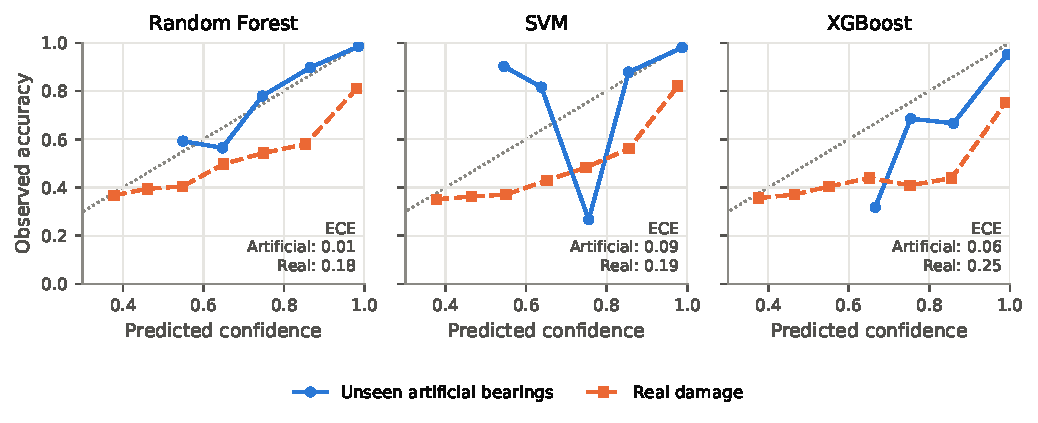
\includegraphics[width=\textwidth]{fig2_reliability}
  \caption{Reliability diagrams (raw probabilities) for unseen artificial bearings (leave one bearing out) and for
    real damage (pooled over 105 rotations). Bins with fewer than 20 windows are omitted. Dotted line: perfect
    calibration. Models that are close to calibrated on unseen artificial bearings are overconfident on real damage
    (ECE 0.18--0.25). The SVM's in-domain dip at 0.75 confidence comes from one held-out artificial bearing (KI01),
    which contributes 80 of that bin's 131 windows, all misclassified.}
  \label{fig:reliability}
\end{figure*}

\subsection{Conformal prediction under-covers}

Split conformal prediction with a nominal coverage of 0.90 reaches 0.65--0.68 on real damage (Table~\ref{tab:main}),
and even the upper ends of the intervals (0.84--0.87) stay below nominal. Mean prediction-set sizes are below
one (0.90--0.96 classes, means over rotations), so some sets are empty: 83--89\,\% of sets contain a single class, and 25--27\,\% of those single-class sets are wrong.
Class-conditional (Mondrian) conformal prediction is no better (coverage 0.63--0.64, means over rotations).

\subsection{Silent bearings}
\label{sec:silent}

Fig.~\ref{fig:perbearing} shows that the failures concentrate on a few bearings. Two outer-race bearings, KA15 and
KA22, are almost never recognised (accuracy 0.02--0.07), and two inner-race bearings, KI16 and KI17, are recognised in
only 29--44\,\% of windows. The models remain confident on all four: mean confidence is 0.69--0.94, and 0.83--0.93
for the two outer-race bearings. The remaining ten test bearings are recognised in at least 68\,\% of windows.
Confidently misclassified bearings are rare among unseen source bearings---none for Random Forest and XGBoost,
one for the SVM (KI01, accuracy 0.00 at mean confidence 0.76)---so calibration fitted on artificial damage has little
chance to anticipate them.

\begin{figure*}[t]
  \centering
  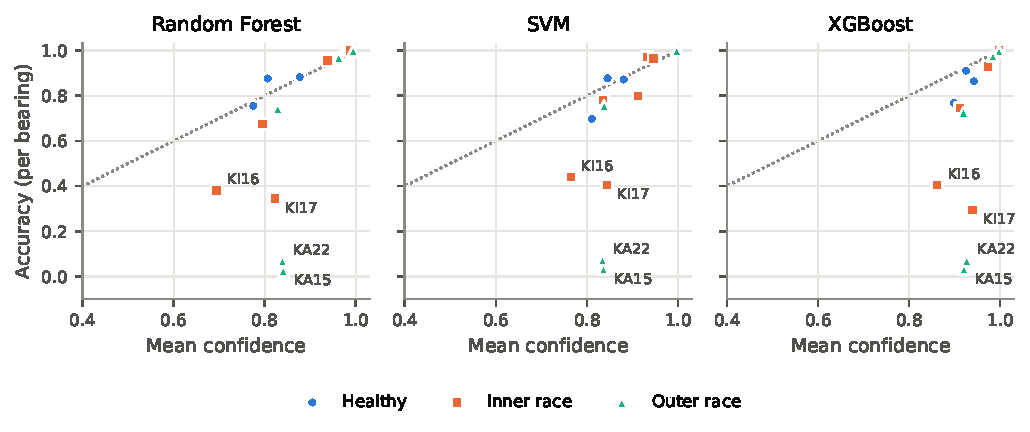
\includegraphics[width=\textwidth]{fig3_per_bearing}
  \caption{Mean confidence and accuracy of each test bearing (11 with real damage, 3 healthy), averaged over 105 rotations (raw
    probabilities). Dotted line: confidence equals accuracy. Four bearings (KA15, KA22: outer race; KI16, KI17: inner
    race) are mostly misclassified while the models remain 69--94\,\% confident on average.}
  \label{fig:perbearing}
\end{figure*}

\subsection{Feature ablation}
\label{sec:ablation}

Adding the five amplitude-based time-domain features (Table~\ref{tab:ablation}) lowers in-domain accuracy from
0.88--0.91 to 0.49--0.77, while accuracy on real damage barely changes (0.65--0.69 vs 0.69). The amplitude features
describe individual bearings rather than damage: unseen healthy bearings in particular are rarely recognised with
them (in-domain healthy accuracy 0.00--0.28), in line with the kurtosis differences between healthy bearings noted in
Section~\ref{sec:splits}. With all features, the in-domain reference is itself poor: for Random Forest and the SVM,
accuracy on real damage is even higher than on unseen artificial bearings (0.69 vs 0.62 and 0.65 vs 0.49), which
hides the artificial-to-real gap. The trustworthiness failure remains: the 5\,\% target is exceeded in
59--92\,\% of the rotations that automate any case, with errors of 0.12--0.17 (means over rotations, as in
Table~\ref{tab:ablation}). Conformal coverage is higher with all features (0.80--0.89), because the prediction sets are
larger (1.3--1.9 classes on average, against 0.9--1.0 with fault-frequency features only).

% Generated by scripts/build_paper_assets.py -- do not edit by hand.
\begin{table}[t]
\centering
\small
\caption{Feature ablation: all nine features vs fault-frequency features only. Means over 105 calibration rotations; temperature scaling; marginal split conformal prediction, nominal coverage 0.90.}
\label{tab:ablation}
\resizebox{\textwidth}{!}{%
\begin{tabular}{llccccccc}
\toprule
\makecell[l]{Features} & Model & \makecell{In-domain\\accuracy} & \makecell{In-domain\\ECE} & \makecell{Real\\accuracy} & \makecell{Real\\ECE} & \makecell{Error at\\5\% target} & \makecell{Runs exceeding\\5\% target} & \makecell{Conformal\\coverage} \\
\midrule
All 9 features & Random Forest & 0.62 & 0.12 & 0.69 & 0.16 & 0.15 & 92\% & 0.85 \\
All 9 features & SVM & 0.49 & 0.37 & 0.65 & 0.16 & 0.12 & 59\% & 0.89 \\
All 9 features & XGBoost & 0.77 & 0.14 & 0.68 & 0.16 & 0.17 & 91\% & 0.8 \\
Fault-frequency only & Random Forest & 0.91 & 0.01 & 0.69 & 0.19 & 0.27 & 100\% & 0.65 \\
Fault-frequency only & SVM & 0.88 & 0.09 & 0.69 & 0.17 & 0.24 & 100\% & 0.68 \\
Fault-frequency only & XGBoost & 0.91 & 0.06 & 0.69 & 0.2 & 0.26 & 100\% & 0.66 \\
\bottomrule
\end{tabular}}
\end{table}


\subsection{1D-CNN baseline}
\label{sec:cnnresults}

The 1D-CNN trained on raw vibration does not generalise to unseen bearings even within the source domain
(Table~\ref{tab:main}). Its leave-one-bearing-out accuracy is 0.46, and its errors are confident (ECE 0.45): every
held-out healthy bearing is classified as damaged at a mean confidence of 0.94--1.00, and four of the five artificial
inner-race bearings are misclassified. The network does learn damage-related patterns---it recognises six of the
seven artificial outer-race bearings, and the real-damage bearings KI14 and KI18 in 93\,\% and 100\,\% of
windows---but with 12 to 14 training bearings it also learns the signatures of individual bearings, in line with the
observation that the number of training bearings limits generalisation \citep{vieira2026}. The random-split sanity
check confirms this. When the test windows come from bearings that are also in the training set, the CNN classifies
98\,\% of them correctly with an ECE of 0.02, as accurately as the feature-based classifiers (0.97--0.98). Holding
out whole bearings costs the feature-based classifiers 6--10 percentage points of accuracy, and the CNN 51 points.

On real damage, the CNN's accuracy is 0.43 [0.16, 0.71]. Because its calibration bearings expose the same problem,
post-hoc calibration makes it cautious rather than reliable: temperature scaling lowers ECE from 0.44 to 0.19, and the
threshold for a 5\,\% error target automates only 13\,\% of cases, yet these still have an error of 0.38. In 55 of the
105 rotations the threshold automates no case at all; in the other 50 the target is exceeded in 43. Even the best
possible threshold automates only 10\,\% of cases.
Marginal conformal prediction reaches a coverage of 0.94, but only by returning 2.5 of the three classes on average;
class-conditional coverage is 0.54. Calibrating on one or two labelled real bearings per class did not help reliably
(error at the 5\,\% target 0.22--0.48 across calibration sets; target met in at most 49\,\% of draws). The CNN's
errors are also of a different kind: only 3\,\% of them are missed faults, the rest being false alarms on healthy
bearings and confusions between fault types. Of the four silent bearings, KA22, KI16 and KI17 remain misclassified
(accuracy 0.02, 0.27 and 0.11), while KA15 is recognised in 48\,\% of windows.

With AdaBN, the network's accuracy on real damage rises from 0.43 to 0.51 [0.24, 0.77], but its confidence does not
become more trustworthy (Table~\ref{tab:main}). The calibration error after temperature scaling is practically
unchanged (0.20 against 0.19), and the error at the 5\,\% target is 0.42. Because the calibration bearings, and with
them the thresholds, are the same as without adaptation, the threshold again automates no case in 55 rotations; in
all of the other 50 it now exceeds the target. Marginal conformal coverage is 0.89, again with large sets (2.3 classes
on average). The gain comes from outer-race and healthy bearings: KA15 and KA30, for example, are recognised in
90\,\% and 96\,\% of windows instead of 48\,\% and 59\,\%. Real inner-race damage, by contrast, is now almost always
called outer-race damage, and more confidently than before: KI04, KI16 and KI17 are classified correctly in 0--6\,\%
of windows at a mean confidence of 0.93--0.97.

\subsection{Calibrating on labelled real bearings}

Table~\ref{tab:realcal} and Fig.~\ref{fig:realcal} compare calibration sets on identical test bearings. With source
(artificial) calibration, the error at the 5\,\% target is 0.26--0.28 and the target is met in at most 1\,\% of draws.
Calibrating on one real bearing per class lowers the error to 0.16--0.19 and meets the target in 29--42\,\% of draws;
two real bearings per class lower it to 0.10--0.11 and meet it in 49--52\,\% of draws. Combining the artificial and
the real calibration bearings lies in between: the error at the 5\,\% target is 0.18--0.19 with one and 0.13--0.14
with two real bearings per class, with 0.58--0.62 and 0.44--0.46 of cases automated, and the target is met in at most
33\,\% of draws.

The improvement comes mainly from caution: the share of cases automated falls from 0.81--0.88 to 0.51--0.52 (one
bearing per class) and 0.35--0.38 (two). Calibration error improves moderately (ECE 0.19--0.22 $\to$ 0.13--0.17 with
two bearings per class), and conformal coverage rises from 0.64--0.67 to 0.84--0.85, still below nominal. Variation
across draws is large (Table~\ref{tab:realcal}), as it depends on which real bearings are available for calibration.

\begin{figure*}[t]
  \centering
  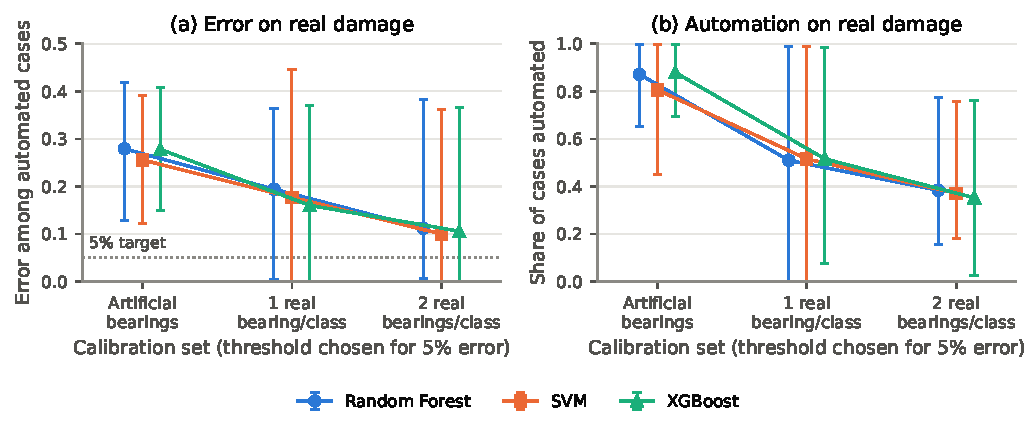
\includegraphics[width=\textwidth]{fig4_real_calibration}
  \caption{Calibrating on a few labelled real-damage bearings (temperature scaling; confidence threshold chosen on
    the calibration set for 5\,\% error). (a) Error among automated real-damage cases; (b) share of real-damage cases
    automated. Points: mean over draws; bars: 2.5th--97.5th percentile over draws (50 draws per real-bearing setting;
    artificial values pooled over all 100).}
  \label{fig:realcal}
\end{figure*}

% Generated by scripts/build_paper_assets.py -- do not edit by hand.
\begin{table*}[t]
\centering
\small
\resizebox{\textwidth}{!}{%
\begin{tabular}{llccccc}
\toprule
Model & Calibrated on & \makecell{Error at\\5\% target} & \makecell{Draws meeting\\5\% target} & Automated & ECE & \makecell{Conformal\\coverage} \\
\midrule
Random Forest & Artificial bearings & 0.28 [0.13, 0.42] & 0\% & 0.87 [0.65, 1.00] & 0.21 [0.10, 0.33] & 0.64 [0.49, 0.80] \\
Random Forest & 1 real bearing/class & 0.19 [0.00, 0.36] & 29\% & 0.51 [0.00, 0.99] & 0.20 [0.05, 0.32] & 0.78 [0.52, 0.98] \\
Random Forest & 2 real bearings/class & 0.11 [0.01, 0.38] & 51\% & 0.38 [0.16, 0.77] & 0.17 [0.02, 0.33] & 0.85 [0.57, 0.99] \\
SVM & Artificial bearings & 0.26 [0.12, 0.39] & 1\% & 0.81 [0.45, 1.00] & 0.19 [0.04, 0.33] & 0.67 [0.51, 0.84] \\
SVM & 1 real bearing/class & 0.18 [0.00, 0.45] & 35\% & 0.52 [0.00, 0.99] & 0.18 [0.04, 0.34] & 0.77 [0.45, 0.98] \\
SVM & 2 real bearings/class & 0.10 [0.00, 0.36] & 52\% & 0.37 [0.18, 0.76] & 0.13 [0.04, 0.29] & 0.85 [0.60, 1.00] \\
XGBoost & Artificial bearings & 0.28 [0.15, 0.41] & 0\% & 0.88 [0.70, 1.00] & 0.22 [0.11, 0.32] & 0.65 [0.51, 0.80] \\
XGBoost & 1 real bearing/class & 0.16 [0.00, 0.37] & 42\% & 0.52 [0.08, 0.99] & 0.19 [0.07, 0.33] & 0.79 [0.54, 0.97] \\
XGBoost & 2 real bearings/class & 0.11 [0.00, 0.37] & 49\% & 0.35 [0.03, 0.76] & 0.16 [0.06, 0.31] & 0.84 [0.58, 0.99] \\
\bottomrule
\end{tabular}}
\caption{Calibrating on artificial bearings vs one or two labelled real bearings per class (fault-frequency features, temperature scaling). Mean [2.5th, 97.5th percentile] over 50 draws per setting; artificial-bearing values pooled over all 100 draws. Within each draw, all settings are scored on the same test bearings. Draws meeting the target count only draws that automated at least one case.}
\label{tab:realcal}
\end{table*}


\subsection{Other operating conditions}
\label{sec:conditions}

Table~\ref{tab:conditions} repeats the evaluation at the three other operating conditions, with the same bearing
splits. At lower load torque the results are almost identical to the main condition: unseen artificial bearings are
classified with accuracy 0.81--0.94, real damage with 0.71, the 5\,\% target is exceeded in every rotation with
an error of 0.25--0.27, and conformal coverage is 0.64--0.68.

At lower radial force and lower speed, the fault-frequency features separate the classes less well even on artificial
damage (in-domain accuracy 0.70--0.76 and 0.57--0.69). The models are then less confident, and the failure is milder
but still present: the error at the 5\,\% target is 0.15--0.21 and 0.10--0.12, the target is exceeded in 88--99\,\% and
68--83\,\% of the rotations that automate any case, and conformal coverage reaches 0.80--0.86, with intervals that include the nominal 0.90.

KA15 and KA22 are misclassified at every condition (mean accuracy over the three models at most 0.41). KI17 is
misclassified at the main condition, at low torque and at 900\,rpm, and KI16 at the main condition and at 900\,rpm;
at low torque KI16 is recognised in 56\,\% of windows. The nature of the errors,
however, depends on the condition. Where the features are strong, most errors are missed faults (62--77\,\% of
errors at the main and low-torque conditions). At lower radial force and lower speed, false alarms on healthy bearings
also occur---healthy bearing K006, for example, is classified as damaged in 92\,\% of its windows at 400\,N---and missed
faults account for 20--27\,\% and 45--50\,\% of errors.

% Generated by scripts/build_paper_assets.py -- do not edit by hand.
\begin{table*}[t]
\centering
\small
\resizebox{\textwidth}{!}{%
\begin{tabular}{llcccccc}
\toprule
Condition & Model & \makecell{In-domain\\accuracy} & \makecell{Real\\accuracy} & \makecell{Error at\\5\% target} & \makecell{Runs exceeding\\5\% target} & \makecell{Conformal\\coverage} & \makecell{Missed faults\\(share of errors)} \\
\midrule
1500 rpm, 0.7 Nm, 1000 N (main) & Random Forest & 0.91 & 0.69 [0.52, 0.86] & 0.27 [0.10, 0.46] & 100\% & 0.65 [0.43, 0.84] & 0.67 \\
1500 rpm, 0.7 Nm, 1000 N (main) & SVM & 0.88 & 0.69 [0.50, 0.86] & 0.24 [0.07, 0.45] & 100\% & 0.68 [0.45, 0.87] & 0.62 \\
1500 rpm, 0.7 Nm, 1000 N (main) & XGBoost & 0.91 & 0.70 [0.52, 0.85] & 0.26 [0.09, 0.44] & 100\% & 0.67 [0.45, 0.85] & 0.68 \\
1500 rpm, 0.1 Nm, 1000 N & Random Forest & 0.94 & 0.71 [0.53, 0.87] & 0.27 [0.11, 0.46] & 100\% & 0.64 [0.41, 0.84] & 0.77 \\
1500 rpm, 0.1 Nm, 1000 N & SVM & 0.81 & 0.71 [0.52, 0.87] & 0.25 [0.08, 0.44] & 100\% & 0.68 [0.42, 0.89] & 0.69 \\
1500 rpm, 0.1 Nm, 1000 N & XGBoost & 0.94 & 0.71 [0.54, 0.87] & 0.26 [0.09, 0.44] & 100\% & 0.67 [0.43, 0.85] & 0.73 \\
1500 rpm, 0.7 Nm, 400 N & Random Forest & 0.76 & 0.66 [0.52, 0.82] & 0.17 [0.02, 0.39] & 98\% & 0.80 [0.56, 0.96] & 0.26 \\
1500 rpm, 0.7 Nm, 400 N & SVM & 0.70 & 0.65 [0.45, 0.81] & 0.21 [0.02, 0.46] & 99\% & 0.80 [0.56, 0.95] & 0.20 \\
1500 rpm, 0.7 Nm, 400 N & XGBoost & 0.74 & 0.67 [0.52, 0.82] & 0.15 [0.00, 0.36] & 88\% & 0.82 [0.59, 0.96] & 0.27 \\
900 rpm, 0.7 Nm, 1000 N & Random Forest & 0.69 & 0.61 [0.44, 0.78] & 0.11 [0.01, 0.33] & 79\% & 0.85 [0.65, 0.99] & 0.50 \\
900 rpm, 0.7 Nm, 1000 N & SVM & 0.57 & 0.61 [0.44, 0.78] & 0.10 [0.01, 0.30] & 68\% & 0.86 [0.64, 0.99] & 0.45 \\
900 rpm, 0.7 Nm, 1000 N & XGBoost & 0.68 & 0.61 [0.45, 0.77] & 0.12 [0.01, 0.33] & 83\% & 0.85 [0.66, 0.97] & 0.48 \\
\bottomrule
\end{tabular}}
\caption{All four Paderborn operating conditions (shaft speed, load torque, radial force), with the same bearing splits. Fault-frequency features, temperature scaling. Real damage: mean [95\,\% interval] from 2,000 bootstrap draws. Missed faults: share of real-damage errors that call a damaged bearing healthy.}
\label{tab:conditions}
\end{table*}



\subsection{Adaptive demodulation band}
\label{sec:adaptive}

Selecting the demodulation band with the fast kurtogram (Section~\ref{sec:features}) did not recover the silent
bearings; it lowered accuracy considerably. The kurtogram chose the band from 10.7 to 21.3\,kHz in 70\,\% of windows,
and this was the most frequent choice for 22 of the 29 bearings, all six healthy bearings included, so it reflects
impulsive content of the test rig rather than bearing damage. In the selected bands the fault peaks of most damaged
bearings weaken or disappear---the outer-race peak of artificial bearing KA07, for example, falls from 16.2 to 1.3
times the noise floor (medians over windows)---and a clear peak remains only for KA01 and for the two bearings whose
band lies near 10\,kHz (KI01 and KI18). The four silent bearings gain no peak (1.8--2.2 times the noise floor at
their fault frequency). Accuracy drops to 0.32--0.36 on unseen artificial bearings and to 0.41--0.43 on real damage
(main condition, temperature scaling). An earlier, simpler selection by spectral kurtosis with a fixed 4\,kHz band
width gave the same picture. The fixed 2--10\,kHz band is therefore the better choice for these signals. A band chosen
by another criterion might still reveal the silent bearings, but neither selection gives evidence for it.

\section{Discussion}
\label{sec:discussion}

For the feature-based models, confidence that was close to calibrated on unseen artificial bearings did not carry over
to real damage: confidence thresholds, post-hoc calibration and conformal prediction all failed in the same direction,
towards overconfidence. Because every bearing belongs to exactly one split, the 5\,\% target is exceeded in all 105
rotations at the main condition, and even the lower ends of the bootstrap intervals over test bearings lie above it,
this is a property of the shift rather than of a particular choice of bearings. The 1D-CNN failed earlier, already on
unseen artificial bearings. The following subsections explain why confidence fails, what this means for calibration,
conformal prediction and practice, and where the study is limited.

\subsection{Why confidence fails on real damage}

The failures are not spread evenly over the real-damage bearings; they concentrate on four of them
(Section~\ref{sec:silent}). Their envelope spectra explain why. For the outer-race bearings KA15 and KA22, the peak at
the outer-race fault frequency is only 2.2 times the spectrum's noise floor (median over windows), and for the
inner-race bearing KI17 the peak at the inner-race frequency is also 2.2. Healthy bearings reach 1.5--2.6 and
1.6--2.1 on the same two features, whereas every artificially damaged bearing reaches at least 5.2 (outer race) or
3.8 (inner race). In the features the models see, these damaged bearings look healthy, and the models classify them
as healthy: 79--85\,\% of windows for KA15 and KA22, 58--70\,\% for KI17. KI16 shows a weak peak at the
\emph{outer}-race frequency (3.2) alongside a weak inner-race peak (2.8), and its windows are split between the two
fault classes.

This has two consequences. First, where the features separate the classes well, the dominant error is the most
dangerous one, a missed fault: at the main condition 62--68\,\% of all errors on real damage declare a damaged
bearing healthy, and 72--74\,\% of the errors made automatically at the 5\,\% target do; at low torque the share is
69--77\,\%. At lower radial force and lower speed, false alarms on healthy bearings are also common, and missed faults
account for only 20--27\,\% and 45--50\,\% of the errors (Section~\ref{sec:conditions}). Second, the models' confidence is not unreasonable given their inputs---a
spectrum without a fault peak \emph{is} typical of a healthy bearing in the training data. No post-hoc calibration
fitted on artificial damage can detect this, because artificial damage always produces a clear peak, and the
calibration set therefore never contains a damaged bearing that looks healthy. The shift is not a gradual drift of
the feature distribution that calibration could absorb; it introduces a type of case the source domain lacks.

The silence is not an artefact of one operating condition: KA15 and KA22 are misclassified at all four conditions,
KI17 at three and KI16 at two. Why the real damage is silent is a separate question that our data cannot settle. The documented
damage does not explain it: the silent bearings include fatigue pitting and an indentation (KA15), and KI16 has the
largest documented extent of all real bearings (level 3), whereas KA04, with the same damage mode and extent as KA22,
shows a clear peak (16.8 times the noise floor). One
explanation is that the damage produces weaker or less regular impacts than a sharp artificial defect; another is
that its impacts excite resonances outside the fixed 2--10\,kHz band. Selecting the band with the fast kurtogram did not
support the second explanation (Section~\ref{sec:adaptive}): the band it selected was dominated by impulsive content
present in healthy bearings as well, and the silent bearings stayed indistinguishable from healthy ones.

Our accuracy on real damage agrees with the dataset authors' own test: trained on artificially damaged bearings, their
classifiers reached 62--75\,\% on real damage with vibration features \citep{lessmeier2016}. Trained and tested on
different real-damage bearings, with time-, frequency- and wavelet-packet features, they reached up to 98\,\%,
recognising KA15 and KA22. The damage is therefore present in the vibration signal; what fails is the transfer of
features and confidence learned from artificial damage.

The 1D-CNN fails in a different way (Section~\ref{sec:cnnresults}). With the raw signal as input and only 12 to 14
training bearings, it partly recognises bearings by characteristics unrelated to their damage, so its confidence is
already misleading on unseen artificial bearings, and on real damage it raises false alarms far more often than it
misses faults. Unlike the failure of the feature-based models, which appears only after the shift, this problem is
visible in a validation by bearing. A random split of windows, which places windows of the same bearings in both
training and test sets, hides it completely: there the CNN is as accurate and as well calibrated as the feature-based
models (Section~\ref{sec:cnnresults}), in line with what \citet{vieira2026} found across several datasets.
Unsupervised domain adaptation did not repair the network's confidence either. AdaBN raised its accuracy on real
damage, but by moving its decisions rather than by telling it when they are wrong: it traded errors on outer-race and
healthy bearings for confident errors on inner-race bearings. Like other unsupervised adaptation methods, it aligns
the overall statistics of the two domains without any information on which target predictions are correct.

\subsection{Calibration in-domain does not imply calibration after the shift}

On unseen artificial bearings, the feature-based models are close to calibrated (ECE 0.01--0.09) and automate 81--91\,\% of cases
at or below 5\,\% error. On real damage, the same models are overconfident (ECE 0.17--0.20 after temperature scaling) and
can automate only 25--30\,\% of cases at that error even with a threshold chosen on the test data. A validation that
holds out artificial bearings---even one done carefully by bearing---would thus give a misleading picture of how the
system behaves in service.

The other operating conditions add a less intuitive observation: the better the features separate the classes on
artificial damage, the more misleading the confidence on real damage. At the main and low-torque conditions, where
in-domain accuracy is highest (0.81--0.94), the 5\,\% target is exceeded in every rotation. At lower radial force and
lower speed, in-domain accuracy is only 0.57--0.76, the models are less confident, and the error at the 5\,\% target
is lower (0.10--0.21), although still above the target in 68--99\,\% of the rotations that automate any case. A model that relies on a clear
fault signature confidently predicts ``healthy'' when that signature is missing, and a missing signature is exactly what
the silent bearings present. This mirrors findings on dataset shift in general machine learning \citep{ovadia2019},
here for a physically meaningful shift in a mechanical system.

\subsection{Conformal prediction under the shift}

The coverage guarantee of split conformal prediction assumes that calibration and test data are exchangeable, and the
artificial-to-real shift breaks this assumption. Coverage fell to 0.65--0.68 against a nominal 0.90, and the
prediction sets offered little warning: most contained a single class. Class-conditional conformal prediction did not
help (0.63--0.64). This differs from \citet{gonzalezgarcia2026}, where class-conditional thresholds partly repaired a
coverage failure caused by different class proportions between calibration and test recordings. Here the problem is
not the proportions but the content of a class: the real-damage bearings of a class do not resemble its artificial
calibration bearings. Weighted conformal prediction \citep{tibshirani2019} could in principle correct for covariate
shift, but it requires estimating how the test inputs differ from the calibration inputs, and the silent bearings
differ precisely by looking like another class.

\subsection{Implications for practice}

Our results suggest four recommendations for deploying automated bearing diagnosis.
\begin{enumerate}[nosep]
  \item \textbf{Do not set automation thresholds on artificial damage alone.} A threshold that gave 5\,\% error on
        held-out artificial bearings gave 24--27\,\% error on real damage.
  \item \textbf{Calibrate on labelled real bearings whenever possible, and expect to automate less.} Two real bearings
        per class reduced the error at the 5\,\% target from about 0.27 to 0.10--0.11, while the share of automated
        cases fell from 0.81--0.88 to 0.35--0.38. This is the honest trade-off: a system that knows less should act
        less.
  \item \textbf{Report results per bearing.} Averages over windows hid that the failures came from four bearings, and
        the wide bootstrap intervals show that a different set of test bearings could change the averages
        considerably.
  \item \textbf{Check features and models on unseen bearings.} Amplitude-based features reflected individual
        bearings, including healthy ones, and lowered accuracy on unseen artificial bearings from 0.88--0.91 to
        0.49--0.77; the 1D-CNN reached only 0.46. On real damage, however, no feature set or model we tested gave
        trustworthy confidence, including the network adapted to unlabelled real-damage data.
\end{enumerate}

\subsection{Limitations}
\label{sec:limitations}

The most important limitation is generality. All bearings come from one test rig and are of one type, the real
damage was produced in accelerated lifetime tests and may differ from damage that develops in the field, and bearings
with combined inner- and outer-race damage were excluded; the size of the effects may therefore differ on other
machines. Repeating the evaluation at all four operating conditions of the dataset shows that the failure is not tied
to one condition, but the experiment with labelled real bearings for calibration, the feature ablation, the adaptive
band and the 1D-CNN were run at the main condition only.

The number of bearings is small---11 with real damage and 6 healthy---so the bootstrap intervals over bearings are
wide. The main conclusions therefore rest on effects that hold in every rotation at the main condition, such as the
5\,\% target being exceeded in all of them, rather than on precise values. Each model was trained with a single random
seed; the rotations and the bootstrap capture variation over bearings, not over training randomness, which matters
most for the 1D-CNN. Conformal calibration is performed on windows, and windows from the same bearing are correlated,
so even the in-domain exchangeability assumption holds only approximately.

Several alternatives remain untested. The features use a fixed demodulation band and window length; the kurtogram
band we tested favoured impulsive content of the test rig, and other criteria for choosing the band were not
explored. The deep-learning baseline is a single architecture trained from scratch with fixed settings, and AdaBN was
the only domain adaptation tested. Pre-training on other data, stronger data augmentation, or adversarial and
discrepancy-based adaptation such as DANN \citep{ganin2016} or Deep CORAL \citep{sun2016} might generalise better
across bearings, although, like AdaBN, they use no labels from the target domain. Whether such methods make the
confidence trustworthy, and not only the accuracy, remains to be tested.

\section{Conclusion}
\label{sec:conclusion}

\todo{About 200 words: main message and practical recommendation.}


\bibliographystyle{plainnat}
\bibliography{references}

\end{document}
